%Este trabalho está licenciado sob a Licença Atribuição-CompartilhaIgual 4.0 Internacional Creative Commons. Para visualizar uma cópia desta licença, visite http://creativecommons.org/licenses/by-sa/4.0/deed.pt_BR ou mande uma carta para Creative Commons, PO Box 1866, Mountain View, CA 94042, USA.

\chapter{Fundamentos sobre funções}\label{cap_funcao}
\thispagestyle{fancy}

\ifispython
\begin{obs}\label{obs:cap_funcao_python}
Ao longo deste capítulo, contaremos com o suporte de alguns códigos \href{https://www.python.org/}{Python} com o seguinte preâmbulo:
\begin{verbatim}
from sympy import *
init_printing()
var('x')
\end{verbatim}
\end{obs}
\fi

\section{Definição e gráfico de funções}\label{cap_funcao_sec_defgrafico}

Uma \pmb{função}\index{função} de um conjunto $D$ em um conjunto $Y$ é uma regra que associa um único elemento $y\in Y$\footnote{$y\in Y$ denota que $y$ é um elemento do conjunto $Y$.} a cada elemento $x\in D$. Costumeiramente, identificamos uma função por uma letra, por exemplo, $f$ e escrevemos $f:D\to Y$, $y=f(x)$, para denotar que a função $f$ toma valores de entrada em $D$ e de saída em $Y$.

O conjunto $D$ de todos os possíveis valores de entrada da função é chamado de \pmb{domínio}\index{domínio}. O conjunto de todos os valores $f(x)$ tal que $x\in D$ é chamado de \pmb{imagem}\index{imagem} da função.

Ao longo do curso de cálculo, as funções serão definidas apenas por expressões matemáticas. Nestes casos, salvo explicitado o contrário, suporemos que a função tem números reais como valores de entrada e de saída. O domínio e a imagem deverão ser inferidos da regra algébrica da função ou da aplicação de interesse.

\begin{ex}
  Determinemos o domínio e a imagem de cada uma das seguintes funções:
  \begin{itemize}
  \item $y=x^2$:
    \begin{itemize}
    \item Para qualquer número real $x$, temos que $x^2$ também é um número real. Então, dizemos que seu domínio (natural)\footnote{O \pmb{domínio natural}\index{domínio!natural} é o conjunto de todos os números reais tais que a expressão matemática que define a função seja possível.} é o conjunto $\mathbb{R} = (-\infty, \infty)$.
    \item Para cada número real $x$, temos $y=x^2\geq0$. Além disso, para cada número real não negativo $y$, temos que $x=\sqrt{y}$ é tal que $y=x^2$. Assim sendo, concluímos que a imagem da função é o conjunto de todos os números reais não negativos, i.e. $[0, \infty)$.
    \end{itemize}
  \item $y=1/x$:
    \begin{itemize}
    \item Lembremos que divisão por zeros não está definida. Logo, o domínio desta função é o conjunto dos números reais não nulos, i.e. $(-\infty, 0)\cup (0, \infty)$.
    \item Primeiramente, observemos que se $y=0$, então não existe número real tal que $0=1/x$. Ou seja, $0$ não pertence a imagem desta função. Por outro lado, dado qualquer número $y\neq 0$, temos que $x=1/y$ é tal que $y=1/x$. Logo, concluímos que a imagem desta função é o conjunto de todos os números reais não nulos, i.e. $(-\infty, 0)\cup (0, \infty)$.
    \end{itemize}
  \item $y=\sqrt{1-x^2}$:
    \begin{itemize}
    \item Lembremos que a raiz quadrada de números negativos não está definida. Portanto, precisamos que:
      \begin{align}
        1-x^2\geq 0 &\Rightarrow x^2 \leq 1\\
                    &\Rightarrow -1 \leq x \leq 1.
      \end{align}
      Donde concluímos que o domínio desta função é o conjunto de todos os números $x$ tal que $-1\leq x \leq 1$ (ou, equivalentemente, o intervalo $[-1, 1]$).
      
      \ifispython
      Com o \href{https://www.sympy.org}{SymPy}, podemos usar o comando
\begin{verbatim}
reduce_inequalities(1-x**2>=0,[x])
\end{verbatim}
      para resolvermos a inequação $1-x^2\geq 0$.
      \fi
    \item Uma vez que $-1 \leq x \leq 1$, temos que $0 \leq 1-x^2 \leq 1$ e, portanto, $0\leq \sqrt{1-x^2} \leq 1$. Ou seja, a imagem desta função é o intervalo $[0, 1]$.
    \end{itemize}
  \end{itemize}
\end{ex}

O \pmb{gráfico}\index{gráfico} de uma função é o conjunto dos pares ordenados $(x, f(x))$ tal que $x$ pertence ao domínio da função. Mais especificamente, para uma função $f:D\to \mathbb{R}$, o gráfico é o conjunto
\begin{equation}
  \{(x, f(x))| x\in D\}.
\end{equation}
O \pmb{esboço do gráfico} de uma função é, costumeiramente, uma representação geométrica dos pontos de seu gráfico em um plano cartesiano.

\begin{ex}\label{ex:grafico}
  A Figura \ref{fig:ex_grafico} mostra os esboços dos gráficos das funções $f(x)=x^2$, $g(x)=1/x$ e $h(x)=\sqrt{1-x^2}$.
  
  \begin{figure}[H]
    \centering
    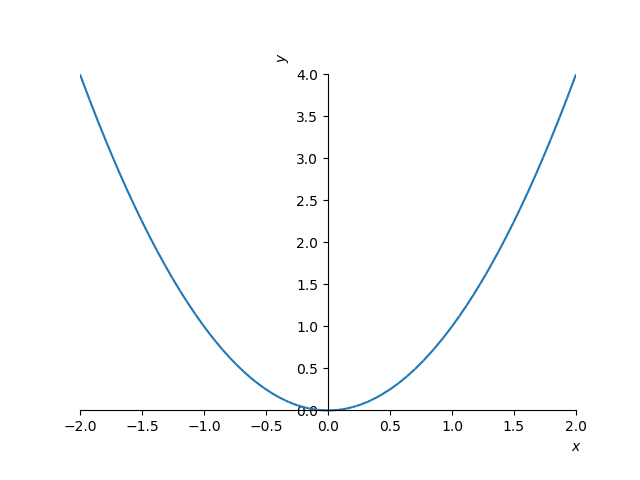
\includegraphics[width=0.3\textwidth]{./cap_funcao/dados/fig_ex_grafico/fig_ex_grafico_x2}~
    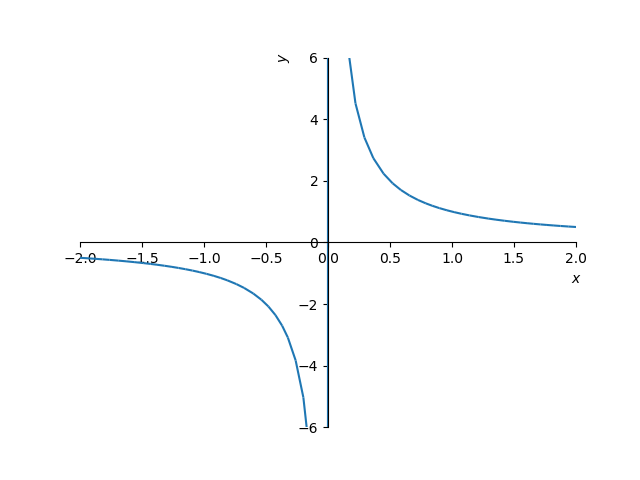
\includegraphics[width=0.3\textwidth]{./cap_funcao/dados/fig_ex_grafico/fig_ex_grafico_1x}~
    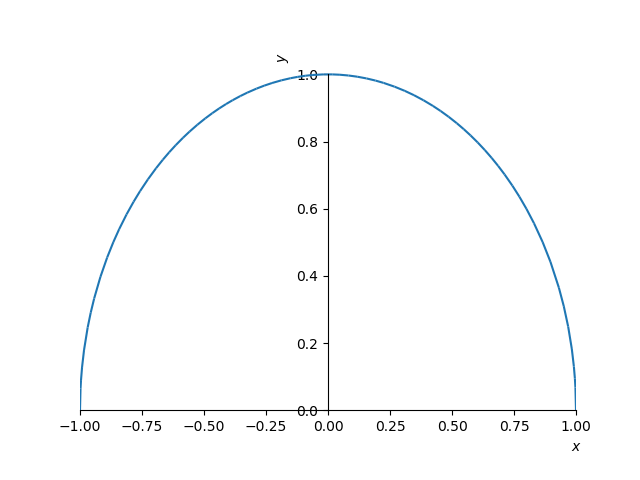
\includegraphics[width=0.3\textwidth]{./cap_funcao/dados/fig_ex_grafico/fig_ex_grafico_s1x2}
    \caption{Esboço dos gráficos das funções $f(x)=x^2$, $g(x)=1/x$ e $h(x)=\sqrt{1-x^2}$ dadas no Exemplo \ref{ex:grafico}.}
    \label{fig:ex_grafico}
  \end{figure}

  \ifispython
  Para plotarmos os gráficos destas funções usando \href{https://www.sympy.org}{SymPy} podemos usar os seguintes comandos:
\begin{verbatim}
plot(x**2,(x,-2,2))
plot(1/x,(x,-1,1),ylim=(-10,10))
plot(sqrt(1-x**2),(x,-1,1))
\end{verbatim}
  \fi
\end{ex}

\subsection*{Exercícios}

\emconstrucao

\section{Função afim}\label{cap_funcao_sec_funafim}

Uma \pmb{função afim}\index{função!afim} é uma função da forma
\begin{equation}
f(x) = mx + b,
\end{equation}
sendo $m$ e $b$ parâmetros\footnote{números reais.} dados. O parâmetro $m$ é chamado de \pmb{coeficiente angular} e o parâmetro $b$ é chamado de \pmb{coeficiente constante}\footnote{Mais corretamente, coeficiente do termo constante.}.

Quando $m=0$, temos uma \pmb{função constante}\index{função!constante} $f(x) = b$. Esta tem domínio $(-\infty, \infty)$ e imagem $\{b\}$. Quando $b=0$, temos uma \pmb{função linear} $f(x)=mx$, cujo domínio é $(-\infty, \infty)$ e imagem é $(-\infty, \infty)$.

Por outro lado, toda função linear com $m\neq 0$ tem $(-\infty, \infty)$ como domínio e imagem.

\begin{ex}\label{ex:funafim}
  A Figura \ref{fig:ex_funafim} mostra esboços dos gráficos das funções afins $f(x)=-5/2$, $f(x)=2$ e $f(x)=2x-1$.
  
  \begin{figure}[H]
    \centering
    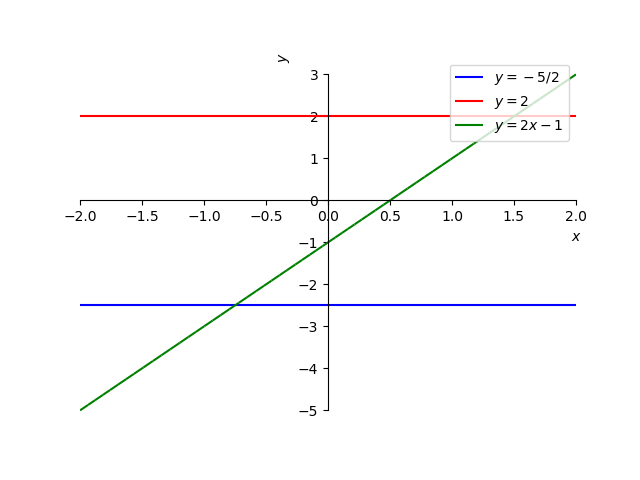
\includegraphics[width=0.7\textwidth]{./cap_funcao/dados/fig_ex_funafim/fig_ex_funafim}
    \caption{Esboços dos gráficos das funções afins $y=-5/2$, $y=2$ e $y=2x-1$ discutidas no Exemplo \ref{ex:funafim}.}
    \label{fig:ex_funafim}
  \end{figure}

  \ifispython
  Com o \verb+Sympy+, podemos plotar os gráficos destas funções com os seguintes comandos\footnote{Veja a Observação \ref{obs:cap_funcao_python}}:
\begin{verbatim}
plot(-5/2,(x,-2,2))
plot(2,(x,-2,2))
plot(2*x-1,(x,-2,2))
\end{verbatim}
  \fi
\end{ex}

O lugar geométrico do gráfico de uma função afim é uma reta (ou linha). O coeficiente angular $m$ controla a inclinação da reta em relação ao eixo $x$\footnote{eixo das abscissas}. Quando $m=0$, temos uma reta horizontal. Quando $m>0$ temos uma reta com inclinação positiva (crescente) e, quando $m<0$ temos uma reta com inclinação negativa.

\begin{ex}\label{ex:funlinear}
  A Figura \ref{fig:ex_funlinear} mostra esboços dos gráficos das funções lineares $f_1(x)=\frac{1}{2}x$, $f_2(x) = x$, $f_3(x) = 2x$, $f_4(x)=-2x$, $f_5(x)=-x$ e $f_6(x)=-\frac{1}{2}x$.
  
  \begin{figure}[H]
    \centering
    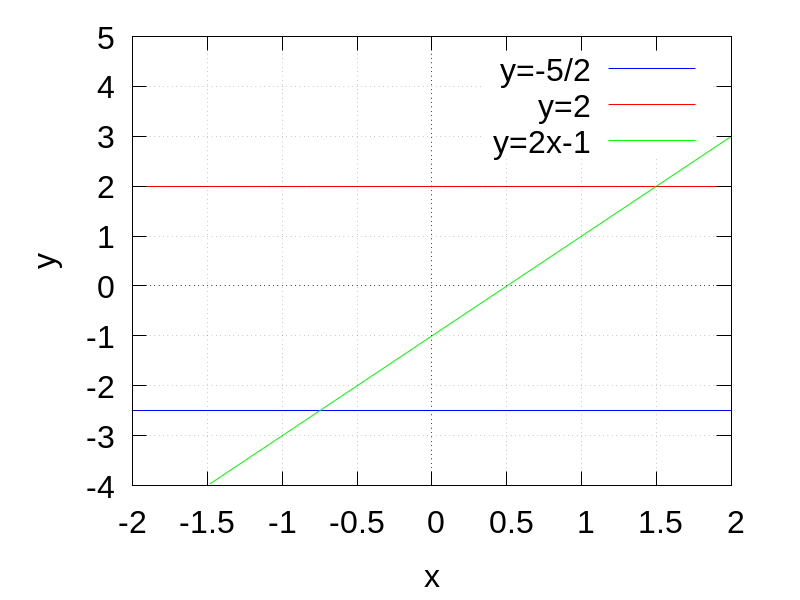
\includegraphics[width=0.7\textwidth]{./cap_funcao/dados/fig_ex_funlinear/fig_ex_funlinear}
    \caption{Esboços dos gráficos das funções lineares discutidas no Exemplo \ref{ex:funlinear}.}
    \label{fig:ex_funlinear}
  \end{figure}

  \ifispython
  Verifique, plotando os gráficos com o \verb+Sympy+!
\end{ex}

\begin{figure}[H]
  \centering
  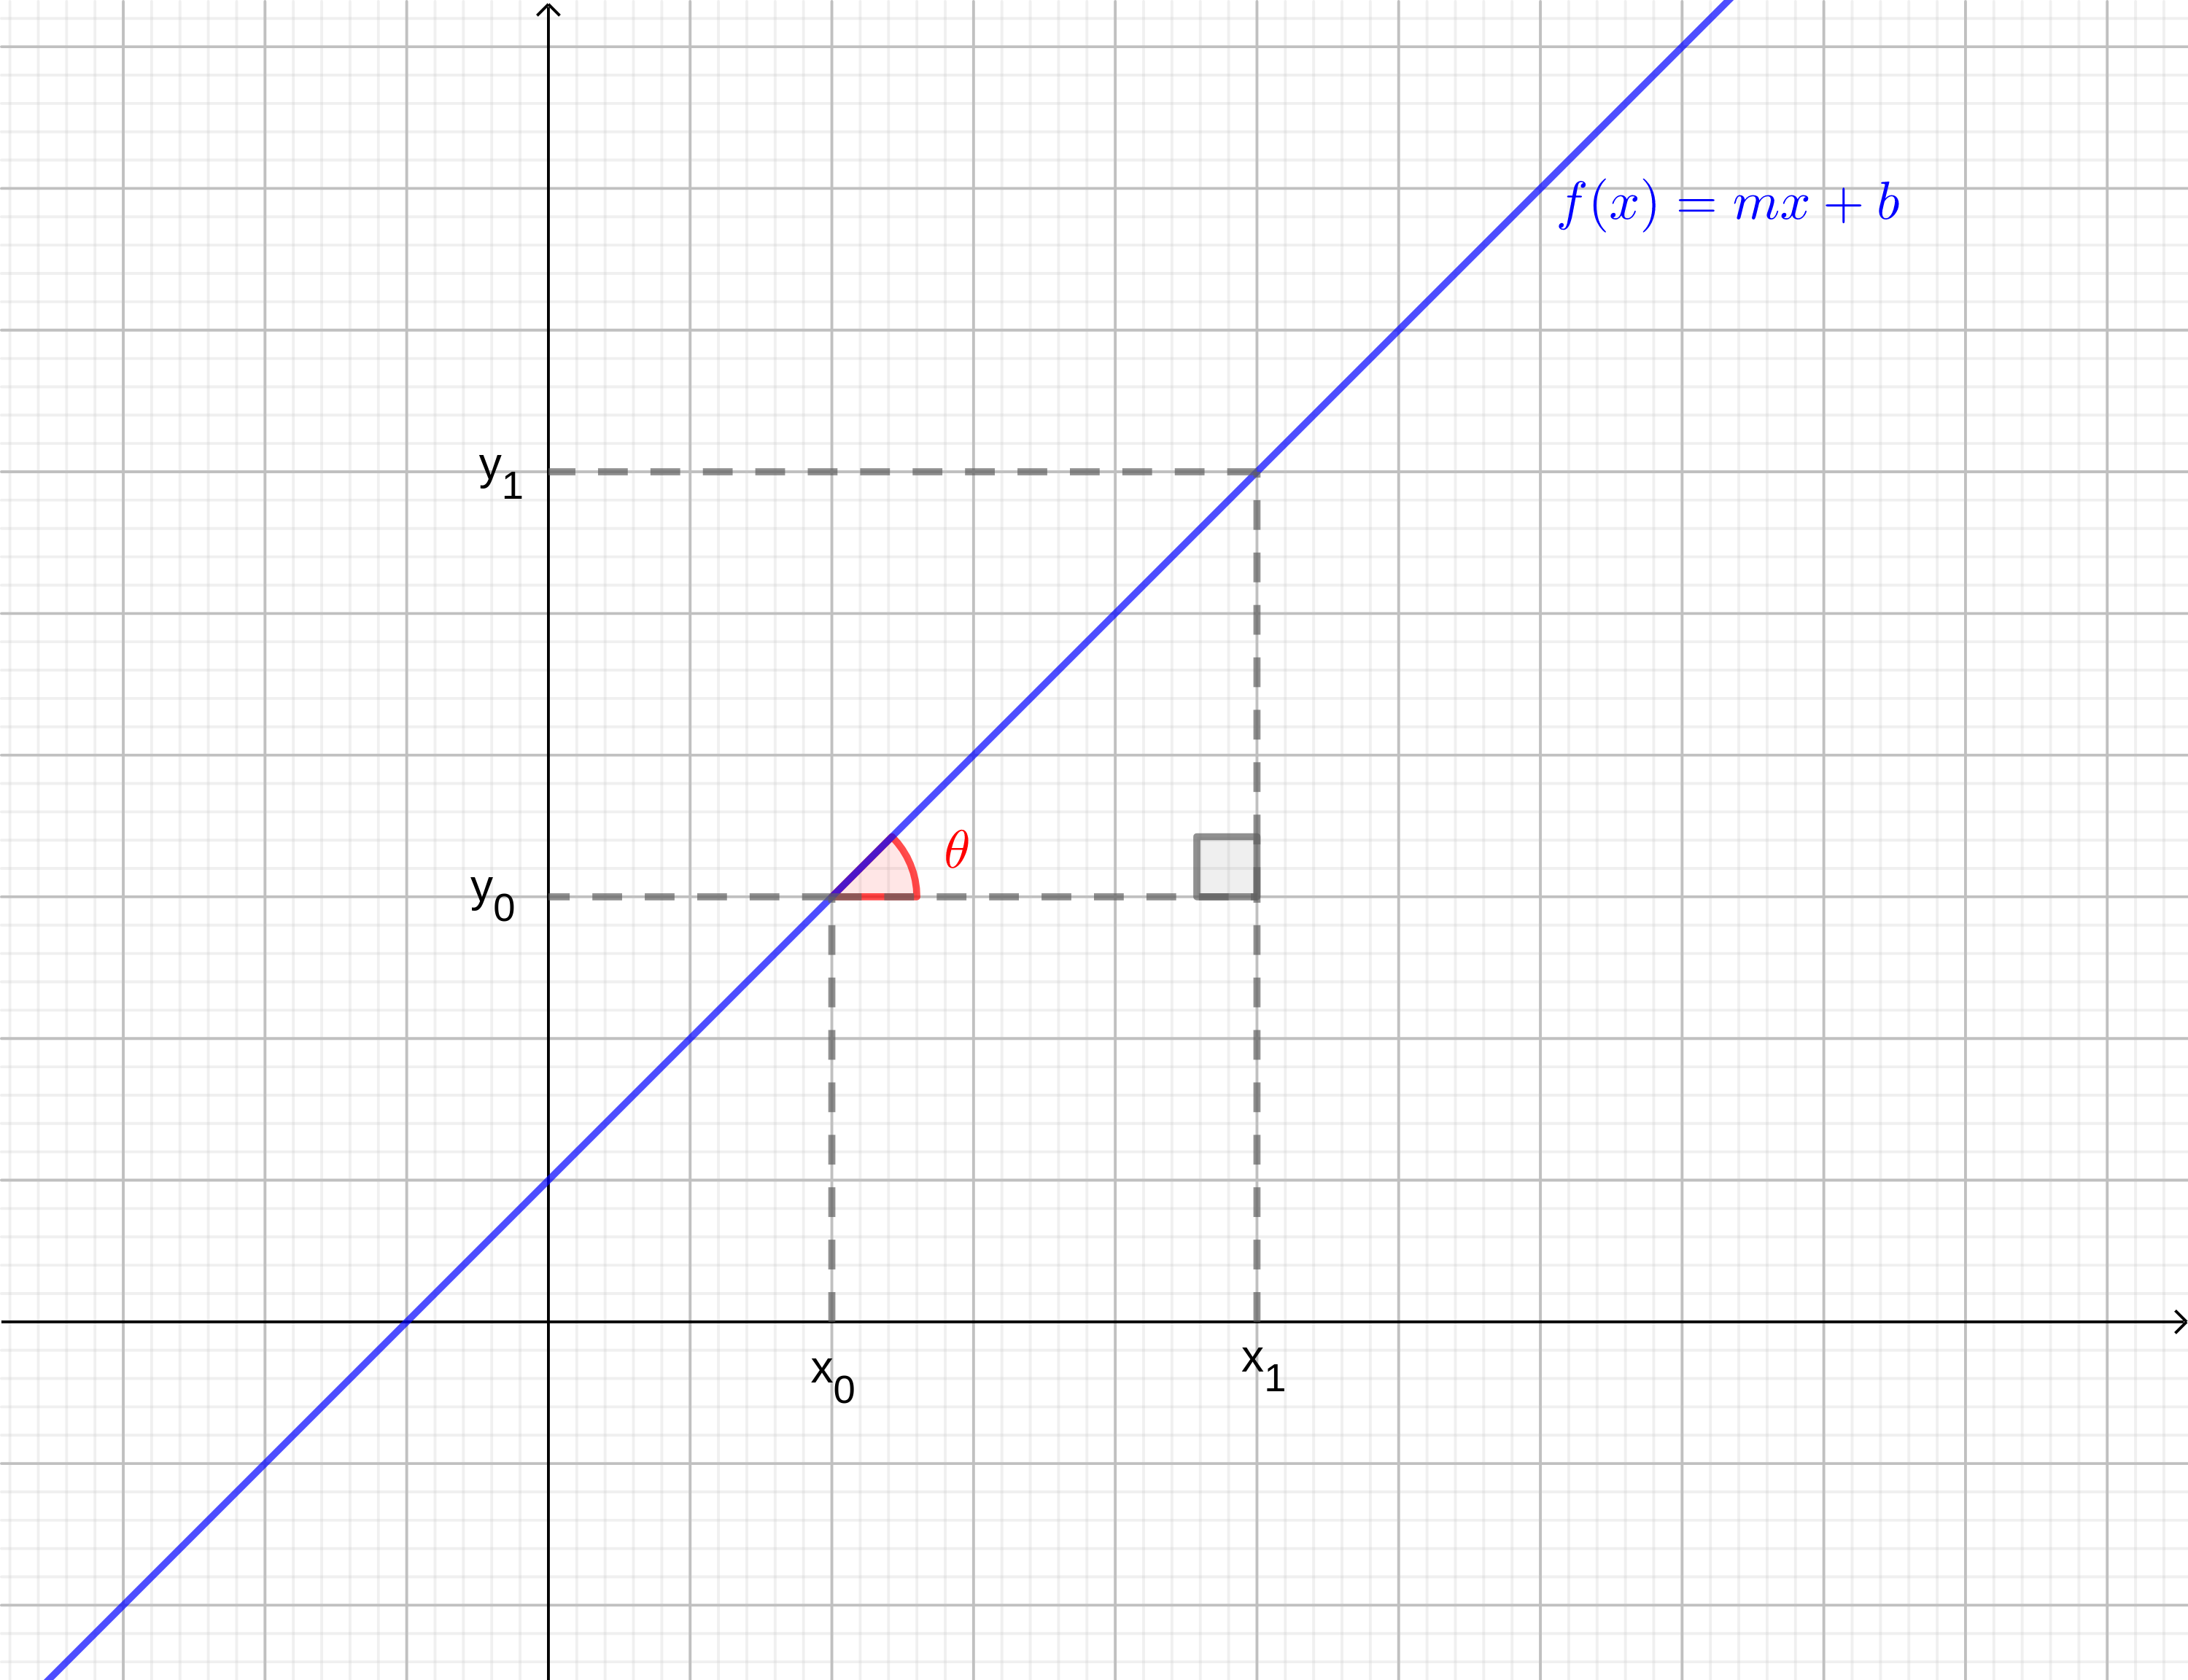
\includegraphics[width=0.7\textwidth]{./cap_funcao/dados/fig_declividade/fig_declividade}
  \caption{Declividade e o coeficiente angular.}
  \label{fig:ex_funlinear}
\end{figure}

A inclinação de uma reta é, normalmente, medida pelo ângulo de declividade (veja a Figura \ref{fig:declividade}). Para definirmos este ângulo, sejam $(x_0, y_0)$ e $(x_1, y_1)$, $x_0<x_1$, pontos sobre uma dada reta, gráfico da função afim $f(x)=mx+b$. O ângulo de declividade (ou, simplesmente, a declividade) da reta é, por definição, o ângulo formado pelo segmento que parte de $(x_0, y_0)$ e termina em $(x_1, y_0)$ e o segmente que parte de $(x_0, y_0)$ e termina em $(x_1, y_1)$. Denotando este ângulo por $\theta$, temos
\begin{align}
  \tg\theta &= \frac{y_1-y_0}{x_1-x_0}\\
            &= \frac{mx_1+b-(mx_0+b)}{x_1-x_0}\\
            &= m,
\end{align}
o que justifica chamar $m$ de coeficiente angular.

Quaisquer dois pontos $(x_0, y_0)$ e $(x_1, y_1)$, com $x_0\neq x_1$, determinam uma única função afim (reta) que passa por estes pontos. Para encontrar a expressão desta função, basta resolver o seguinte sistema linear
\begin{align}
  mx_0 + b &= y_0\\
  mx_1 + b &= y_1
\end{align}
Subtraindo a primeira equação da segunda, obtemos
\begin{equation}
  m(x_0-x_1) = y_0-y_1 \Rightarrow m = \frac{y_0-y_1}{x_0-x_1}.
\end{equation}
Daí, substituindo o valor de $m$ na primeira equação do sistema, obtemos
\begin{equation}
  \frac{y_0-y_1}{x_0-x_1}x_0 + b = y_0 \Rightarrow b = -\frac{y_0-y_1}{x_0-x_1}x_0 + y_0.
\end{equation}
Ou seja, a expressão da função linear (equação da reta) que passa pelos pontos $(x_0, y_0)$ e $(x_1, y_1)$ é
\begin{equation}
  y = \underbrace{\frac{y_0-y_1}{x_0-x_1}}_{m}(x-x_0) + y_0.
\end{equation}

\subsection*{Exercícios resolvidos}

\begin{exeresol}
Trace o esboço da reta que representa o gráfico da função afim $f(x) = -x-1$.  
\end{exeresol}
\begin{resol}
  Para esboçar o gráfico de uma função afim, basta traçarmos a reta que passa por quaisquer dois pontos distintos de seu gráfico. Por exemplo, no caso da função $f(x) = -x -1$, temos
  \begin{center}
  \begin{tabular}[H]{r|c}
    $x$ & $y = -x-1$\\\hline
    -1  & 0\\
    1   & -2\\\hline
  \end{tabular}
\end{center}
Assim sendo, marcamos os pontos $(-1, 0)$ e $(1, -2)$ em um plano cartesiano e traçamos a reta que passa por eles. Veja a Figura \ref{fig:exeresol_funafim_grafico}.

\begin{figure}[H]
  \centering
  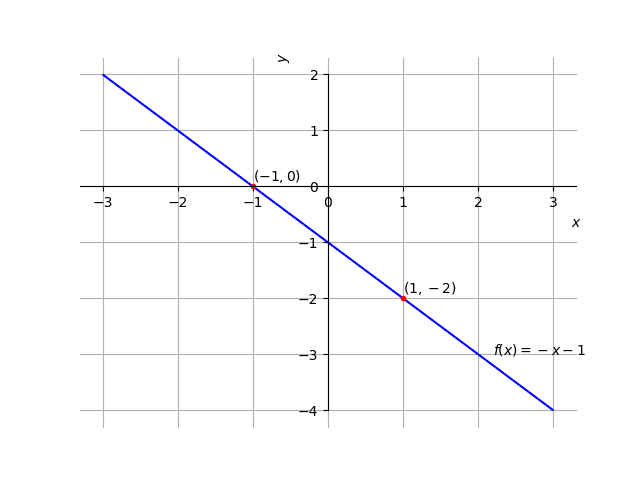
\includegraphics[width=0.7\textwidth]{./cap_funcao/dados/fig_exeresol_funafim_grafico/fig_exeresol_funafim_grafico}
  \caption{Esboço do gráfico da função afim $f(x)=-x-1$.}
  \label{fig:exeresol_funafim_grafico}
\end{figure}

\ifispython
Com o \verb+Sympy+, podemos plotar o gráfico da função $f(x)=-x-1$ com o seguinte comando\footnote{Veja a Observação \ref{obs:cap_funcao_python}}:
\begin{verbatim}
plot(-x-1,(x,-3,3))
\end{verbatim}
\fi
\end{resol}

\subsection*{Exercícios}

\emconstrucao

\section{Função potência}\label{cap_funcao_sec_funpot}

Uma função da forma $f(x)=x^n$, onde $n\neq 0$ é uma constante, é chamada de \pmb{função potência}\index{função!potência}.

Funções potências têm comportamentos característicos, conforme o valor de $n$. Quando $n$ é um inteiro positivo ímpar, seu domínio e sua imagem são $(-\infty, \infty)$. Veja a Figura \ref{fig:funpot_impar}.

\begin{figure}[H]
  \centering
  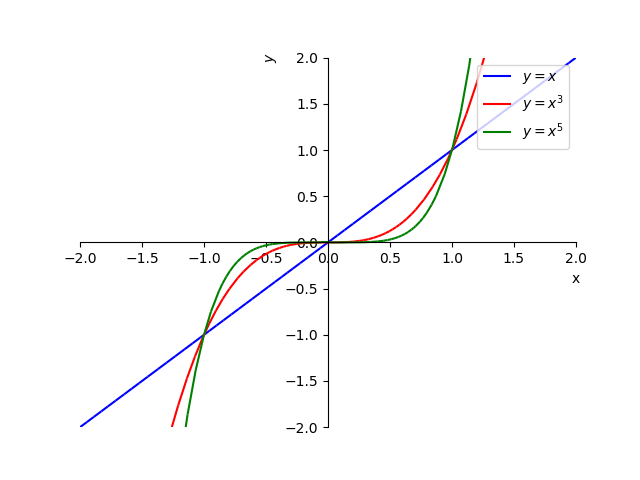
\includegraphics[width=0.7\textwidth]{./cap_funcao/dados/fig_funpot_impar/fig_funpot_impar}
  \caption{Esboços dos gráficos das funções potências $y=x$, $y=x^3$ e $y=x^5$.}
  \label{fig:funpot_impar}
\end{figure}

Funções potências com $n$ positivo par estão definidas em toda parte e têm imagem $[0, \infty)$. Veja a Figura \ref{fig:funpot_par}.

\begin{figure}[H]
  \centering
  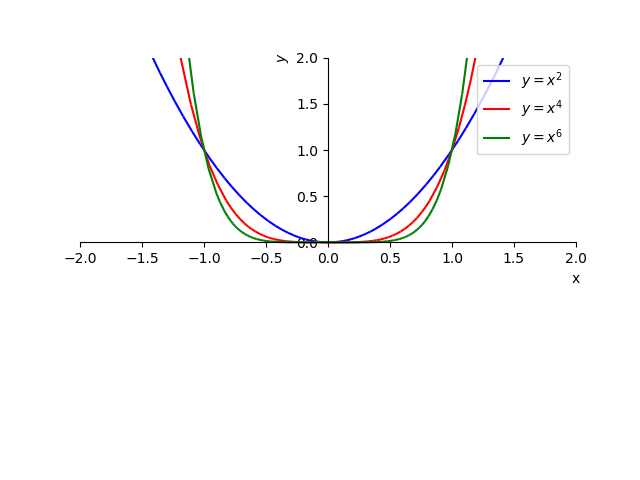
\includegraphics[width=0.7\textwidth]{./cap_funcao/dados/fig_funpot_par/fig_funpot_par}
  \caption{Esboços dos gráficos das funções potências $y=x^2$, $y=x^4$ e $y=x^6$.}
  \label{fig:funpot_par}
\end{figure}

Funções potências com $n$ inteiro negativo ímpar não são definidas em $x=0$, tendo domínio e imagem igual a $(-\infty, 0)\cup (0, \infty)$. Também, quando $n$ inteiro negativo par, a função potência não está definida em $x=0$, tem domínio $(-\infty, 0)\cup (0, \infty)$, mas imagem $(0, \infty)$. Veja a Figura \ref{fig:funpot_negativo}.

\begin{figure}[H]
  \centering
  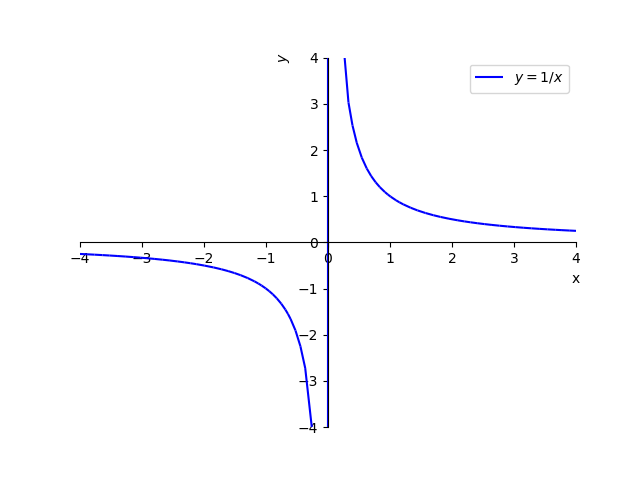
\includegraphics[width=0.5\textwidth]{./cap_funcao/dados/fig_funpot_negativo/fig_funpot_negativo_impar}~
    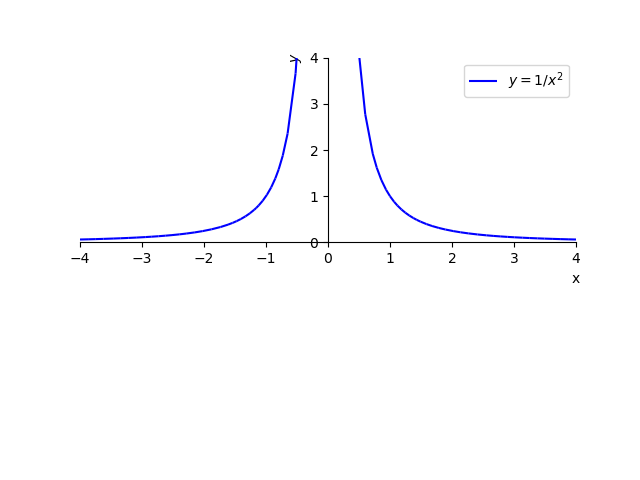
\includegraphics[width=0.5\textwidth]{./cap_funcao/dados/fig_funpot_negativo/fig_funpot_negativo_par}
  \caption{Esboços dos gráficos das funções potências $y=1/x$ (esquerda), $y=1/x^2$ (direita).}
  \label{fig:funpot_negativo}
\end{figure}

Há, ainda, comportamentos característicos quando $n=1/2$, $1/3$, $3/2$ e $2/3$. Veja a Figura \ref{fig:funpot_racional}.

\begin{figure}[H]
  \centering
  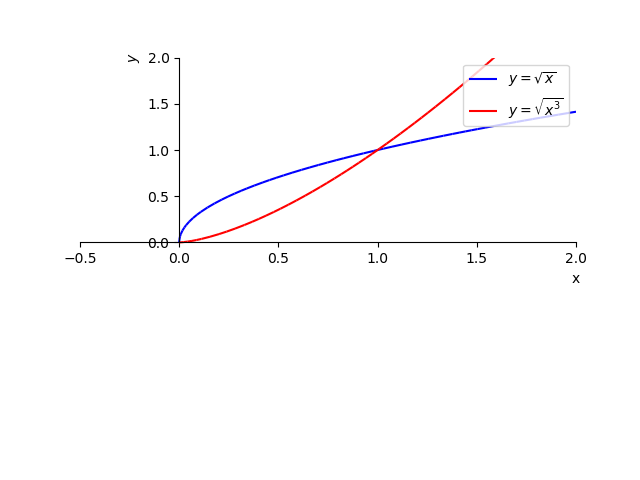
\includegraphics[width=0.5\textwidth]{./cap_funcao/dados/fig_funpot_racional/fig_funpot_racional_par}~
    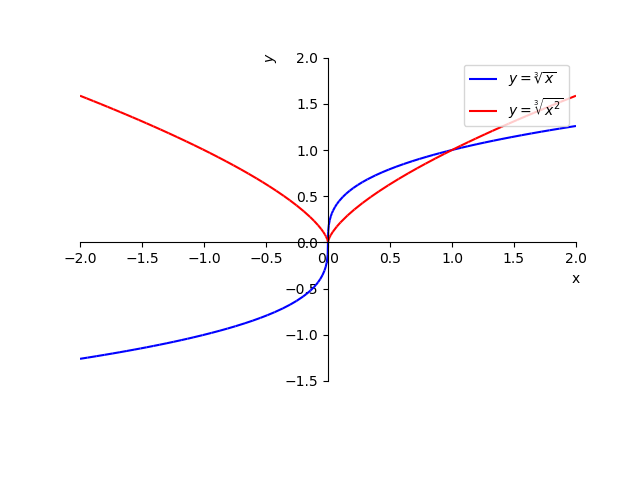
\includegraphics[width=0.5\textwidth]{./cap_funcao/dados/fig_funpot_racional/fig_funpot_racional_impar}
  \caption{Esboços dos gráficos das funções potências. Esquerda $y=\sqrt{x}$ e $y=\sqrt{x^3}$. Direita: $y=\sqrt[3]{x}$ e $y=\sqrt[3]{x^2}$.}
  \label{fig:funpot_racional}
\end{figure}


\subsection*{Exercícios resolvidos}

\emconstrucao

\subsection*{Exercícios}

\emconstrucao

\section{Função polinomial}\label{cap_funcao_sec_funpoli}

Uma {\bf função polinomial}\index{função polinomial} ({\bf polinômio}\index{polinômio}) tem a forma
\begin{equation}
  p(x) = a_nx^n + a_{n-1}x^{n-1} + \cdots + a_1x + a_0,
\end{equation}
onde $a_i$ são coeficientes reais, $a_n\neq 0$ e $n$ é inteiro não negativo, este chamado de {\bf grau do polinômio}\index{grau do polinômio}.

Polinômios são definidos em toda parte\footnote{Uma função é dita ser definida em toda parte quando seu domínio é $(\infty, \infty)$}. Polinômios de grau ímpar tem imagem $(-\infty, \infty)$. Entretanto, a imagem polinômios de grau par dependem de cada caso. Iremos estudar mais propriedades de polinômios ao longo do curso de cálculo. Veja a Figura \ref{fig:poli_graficos}.

\begin{figure}[H]
  \centering
  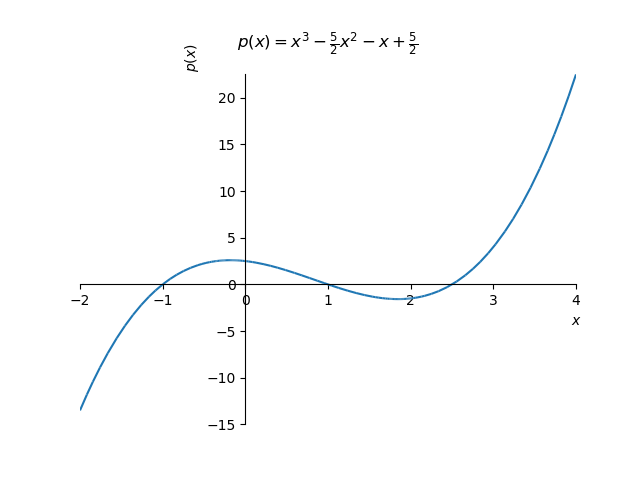
\includegraphics[width=0.5\textwidth]{./cap_funcao/dados/fig_poli_graficos/fig_poli_impar}~
    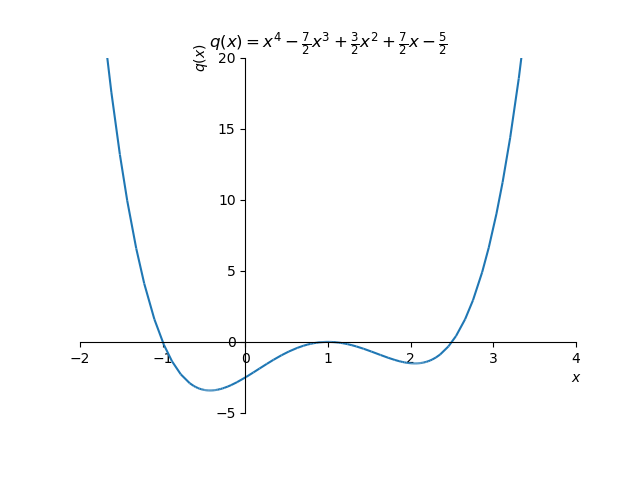
\includegraphics[width=0.5\textwidth]{./cap_funcao/dados/fig_poli_graficos/fig_poli_par}
  \caption{Esboços dos gráficos das funções polinomiais. Esquerda $p(x) = x^{3} - 2.5 x^{2} - 1.0 x + 2.5$. Direita: $q(x) = x^{4} - 3.5 x^{3} + 1.5 x^{2} + 3.5 x - 2.5$.}
  \label{fig:poli_graficos}
\end{figure}

Quando $n=0$, temos um polinômio de grau 0 (ou uma função constante). Quando $n=1$, temos um polinômio de grau 1 (ou, uma função linear). Ainda, quando $n=2$ temos uma {\bf função quadrática}\index{função!quadrática} (ou {\bf polinômio quadrático}\index{polinômio!quadrático}) e, quando $n=3$, temos uma {\bf função cúbica}\index{função!cúbica} (ou {\bf polinômio cúbico}\index{polinômio cúbico}).

\subsection*{Exercícios resolvidos}

\emconstrucao

\subsection*{Exercícios}

\emconstrucao

\subsection{Função racional}\label{cap_funcao_sec_funracio}

Uma {\bf função racional}\index{função!racional} tem a forma
\begin{equation}
  f(x) = \frac{p(x)}{q(x)},
\end{equation}
onde $p(x)$ e $q(x)\not\equiv 0$ são polinômios.

Função racionais não estão definidas nos zeros de $q(x)$. Além disso, suas imagens dependem de cada caso. Estudaremos o comportamento de funções racionais ao longo do curso de cálculo. Veja a Figura \ref{fig:racional_grafico}.

\begin{figure}[H]
  \centering
  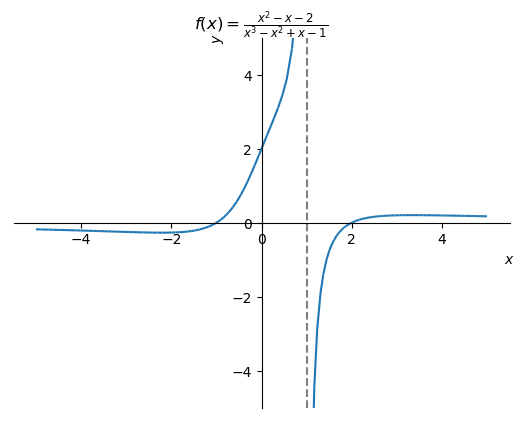
\includegraphics[width=0.8\textwidth]{./cap_funcao/dados/fig_racional_grafico/fig_racional_grafico}
  \caption{Esboço do gráfico da função racional $f(x) = \frac{x^{2} - x - 2}{x^{3} - x^{2} + x - 1}$.}
  \label{fig:racional_grafico}
\end{figure}

\subsection*{Exercícios resolvidos}

\emconstrucao

\subsection*{Exercícios}

\emconstrucao

\section{Categorizações de funções}

\subsection{Funções algébricas}

{\bf Funções algébricas}\index{função!algébrica} são funções definidas a partir de somas, subtrações, multiplicações, divisões ou extração de raízes de funções polinomiais. Estudaremos estas funções ao longo do curso de cálculo.

\subsection{Funções transcendentes}

{\bf Funções transcendentes}{\index{função!transcendente}} são funções que não são algébricas. Como exemplos, temos as funções trigonométricas, exponencial e logarítmica, as quais introduziremos nas próximas seções.

\subsection{Funções definidas por partes}

\pmb{Funções definidas por partes}\index{função!definida por partes} são funções definidas por diferentes expressões matemáticas em diferentes partes de seu domínio.

\begin{ex}\label{ex:funpartes}
  Consideremos a seguinte função definida por partes:
  \begin{equation}
    f(x) = \left\{
      \begin{array}{ll}
        -x &, x<0,\\
        x^2 &, x\geq0
      \end{array}
\right.
\end{equation}
Observemos que tanto o domínio como a imagem desta função são $(-\infty, \infty)$. A Figura \ref{fig:ex_funpartes} mostra o esboço do gráfico desta função.

\begin{figure}[H]
  \centering
  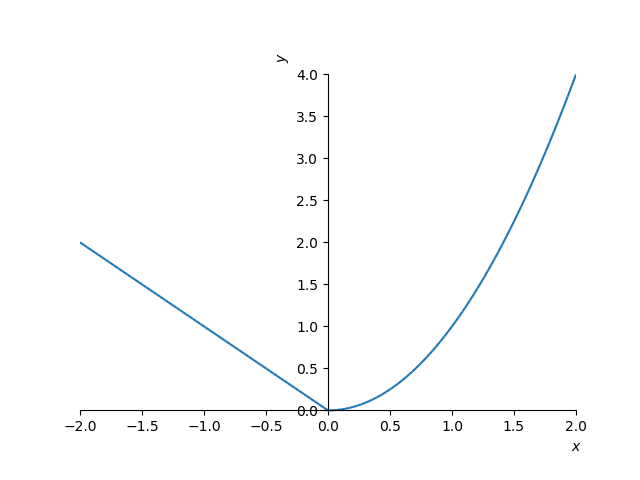
\includegraphics[width=0.7\textwidth]{./cap_funcao/dados/fig_ex_funpartes/fig_ex_funpartes}
  \caption{Esboço do gráfico da função definida por partes $f(x)$ dada no Exemplo \ref{ex:funpartes}.}
  \label{fig:ex_funpartes}
\end{figure}
\end{ex}

Um exemplo de função definida por partes fundamental é a \pmb{função valor absoluto}\index{função!valor absoluto}\footnote{Esta função também pode ser definida por $|x| = \sqrt{x^2}$.}
\begin{equation}
  |x| = \left\{
    \begin{array}{ll}
      x &, x\leq 0\\
      -x &, x<0
    \end{array}
\right.
\end{equation}
Vejamos o esboço do seu gráfico dado na Figura \ref{fig:funabs}.

\begin{figure}[H]
  \centering
  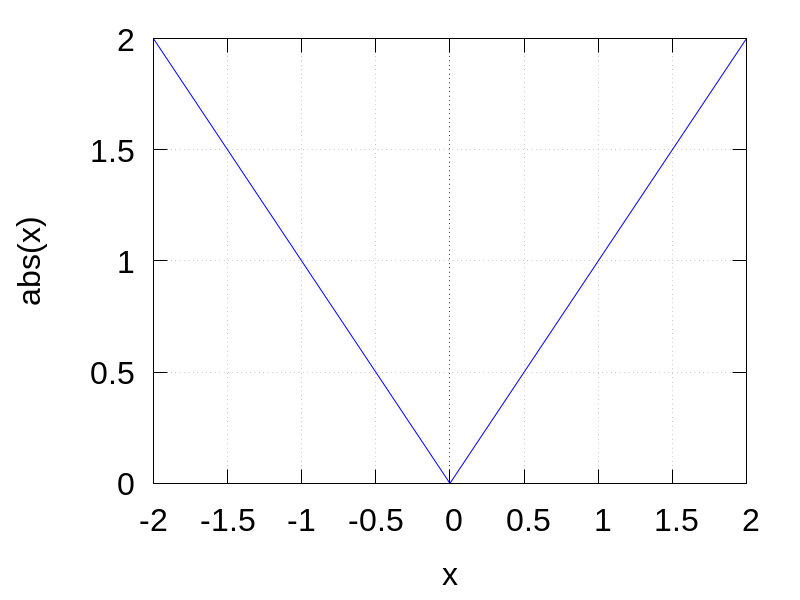
\includegraphics[width=0.7\textwidth]{./cap_funcao/dados/fig_funabs/fig_funabs}
  \caption{Esboço do gráfico da função valor absoluto $y=|x|$.}
  \label{fig:funabs}
\end{figure}

\subsection*{Exercícios resolvidos}

\emconstrucao

\subsection*{Exercícios}

\emconstrucao

\section{Funções trigonométricas}\label{cap_funcao_sec_funtri}

\subsection{Seno e cosseno}

As funções trigonométricas seno $y=\sen(x)$ e cosseno $y=\cos(x)$ podem ser definidas a a partir do círculo trigonométrico (veja a Figura \ref{fig:cos_seno}). Seja $x$ o ângulo\footnote{Em geral utilizaremos a medida em radianos para ângulos.} de declividade da reta que passa pela origem do plano cartesiano (reta $r$ na Figura \ref{fig:cos_seno}). Seja, então, $(a,b)$ o ponto de interseção desta reta com a circunferência unitária\footnote{Circunferência do círculo de raio 1.}. Então, definimos:
\begin{equation}
  \sen(x) = a,\qquad \cos(x) = b.
\end{equation}
A partir da definição, notemos que ambas funções têm domínio $(-\infty, \infty)$ e imagem $[-1, 1]$.

\begin{figure}[H]
  \centering
  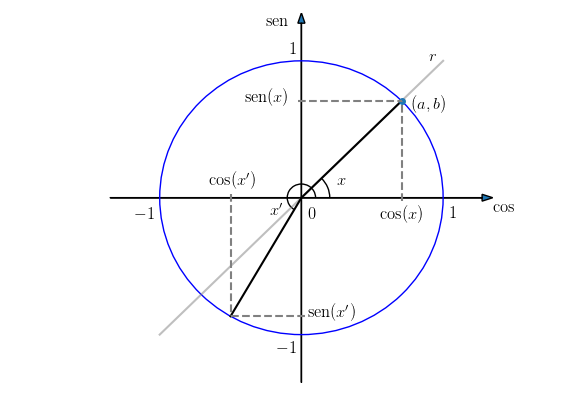
\includegraphics[width=0.8\textwidth]{./cap_funcao/dados/fig_cos_seno/fig_cos_seno}
  \caption{Funções seno e cosseno no círculo trigonométrico.}
  \label{fig:cos_seno}
\end{figure}

Na Figura \ref{fig:cos_seno_valores} podemos extrair os valores das funções seno e cosseno para os ângulos fundamentais. Por exemplo, temos
\begin{align}
  &\sen\left(\frac{\pi}{6}\right) = \frac{1}{2},\qquad \cos\left(\frac{\pi}{6}\right) = \frac{\sqrt{3}}{2},\\
  &\sen\left(\frac{3\pi}{4}\right) = \frac{\sqrt{2}}{2},\qquad \cos\left(\frac{\pi}{4}\right) = -\frac{\sqrt{2}}{2},\\
  &\sen\left(\frac{8\pi}{6}\right) = -\frac{\sqrt{3}}{2},\qquad \cos\left(\frac{8\pi}{6}\right) = -\frac{1}{2},\\
  &\sen\left(\frac{11\pi}{6}\right) = -\frac{1}{2},\qquad \cos\left(\frac{11\pi}{6}\right) = \frac{\sqrt{3}}{2},\\
\end{align}
\ifispython
As funções seno e cosseno estão definidas no \href{https://www.sympy.org}{SymPy} como \verb+sin+ e $\verb+cos+$, respectivamente. Por exemplo, para computar o seno de $\pi/6$, digitamos:
\begin{verbatim}
sin(pi/6)
\end{verbatim}
\fi

\begin{figure}[H]
  \centering
  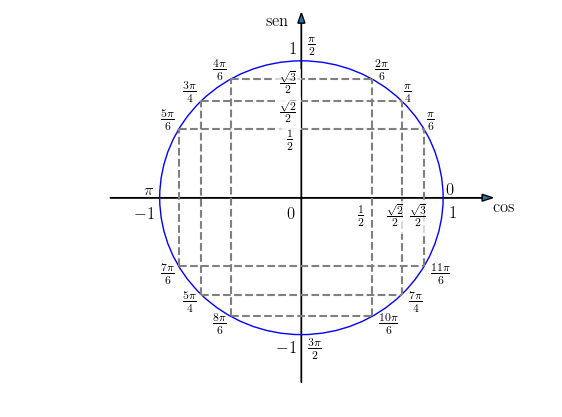
\includegraphics[width=0.8\textwidth]{./cap_funcao/dados/fig_cos_seno_valores/fig_cos_seno_valores}
  \caption{Funções seno e cosseno no círculo trigonométrico.}
  \label{fig:cos_seno_valores}
\end{figure}

Uma {\bf função} $f(x)$ é dita {\bf periódica}\index{função!periódica} quando existe um número $p$, chamado de período da função, tal que
\begin{equation}
  f(x+p) = f(x)
\end{equation}
para qualquer valor de $x$ no domínio da função. Da definição das funções seno e cosseno, notemos que ambas são periódicas com período $2\pi$, i.e.
\begin{equation}
  \sen(x+2\pi) = \sen(x),\qquad \cos(x+2\pi) = \cos(x),
\end{equation}
para qualquer valor de $x$.

Na Figura \ref{fig:cos_seno_graficos}, temos os esboços dos gráficos das funções seno e cosseno.

\begin{figure}[H]
  \centering
  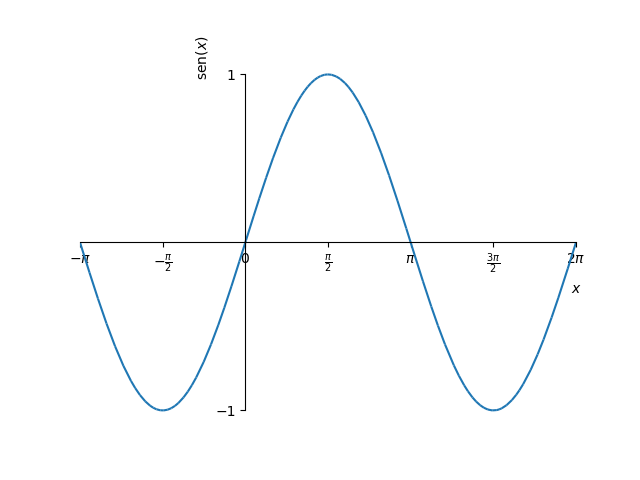
\includegraphics[width=0.5\textwidth]{./cap_funcao/dados/fig_cos_seno_graficos/fig_seno_grafico}~
  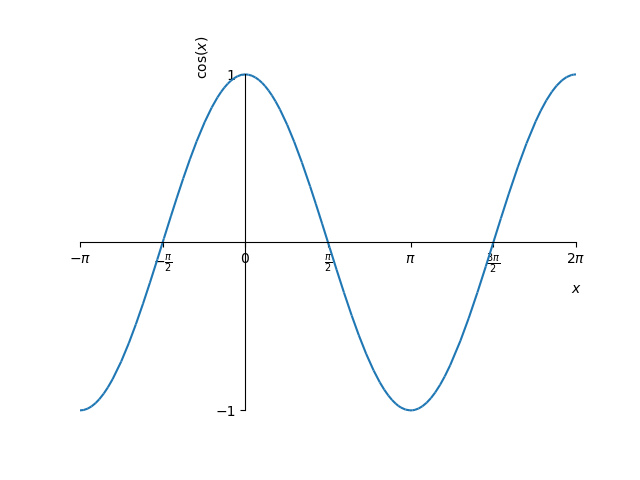
\includegraphics[width=0.5\textwidth]{./cap_funcao/dados/fig_cos_seno_graficos/fig_cosseno_grafico}
  \caption{Esboços dos gráficos das funções seno (esquerda) e cosseno (direita).}
  \label{fig:cos_seno_graficos}
\end{figure}

\subsection{Tangente, cotangente, secante e cossecante}

Das funções seno e cosseno, definimos as funções {\bf tangente}\index{função!tangente}, {\bf cotangente}\index{função!cotangente}, {\bf secante}\index{função!secante} e {\bf cossecante}\index{função!cossecante} como seguem:
\begin{align}
  \tg(x) := \frac{\sen(x)}{\cos(x)},\qquad \cotg(x) := \frac{\cos(x)}{\sen(x)},\\
  \sec(x) := \frac{1}{\cos(x)},\qquad \cosec(x) := \frac{1}{\sen(x)}.
\end{align}

\ifispython
No \href{https://www.sympy.org}{SymPy}, as funções tangente, cotangente, secante e cossecante podem ser computadas com as funções $\verb+tan+$, $\verb+cot+$, $\verb+sec+$ e $\verb+csc+$, respectivamente. Por exemplo, podemos computar o valor de $\cosec(\pi/4)$ com o comando
\begin{verbatim}
csc(pi/4)
\end{verbatim}
\fi

Na Figura \ref{fig:co_tg_graficos}, temos os esboços dos gráficos das funções tangente e cotangente. Observemos que a função tangente não está definida nos pontos $(2k+1)\pi/2$, para todo $k$ inteiro. Já, a função cotangente não está definida nos pontos $k\pi$, para todo $k$ inteiro. Ambas estas funções têm imagem $(-\infty, \infty)$ e período $\pi$.

\begin{figure}[H]
  \centering
  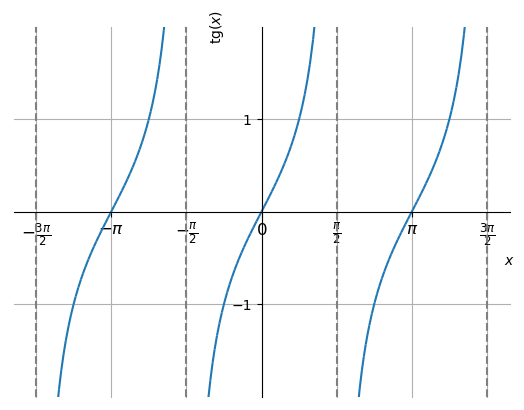
\includegraphics[width=0.5\textwidth]{./cap_funcao/dados/fig_co_tg_graficos/fig_tg_grafico}~
  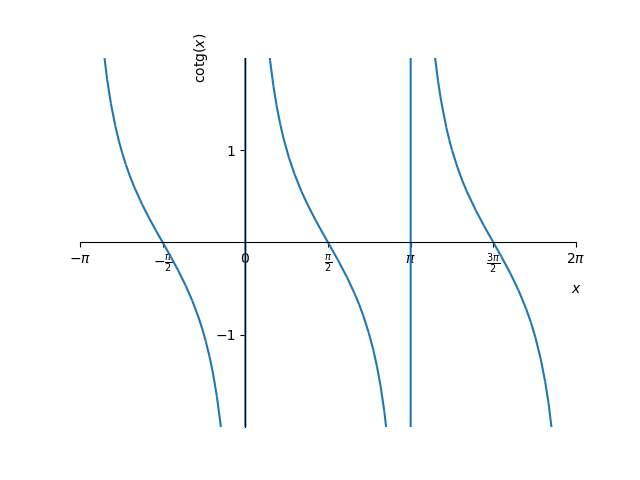
\includegraphics[width=0.5\textwidth]{./cap_funcao/dados/fig_co_tg_graficos/fig_cotg_grafico}
  \caption{Esboços dos gráficos das funções tangente (esquerda) e cotangente(direita).}
  \label{fig:co_tg_graficos}
\end{figure}

Na Figura \ref{fig:co_sec_graficos}, temos os esboços dos gráficos das funções secante e cossecante. Observemos que a função secante não está definida nos pontos $(2k+1)\pi/2$, para todo $k$ inteiro. Já, a função cossecante não está definida nos pontos $k\pi$, para todo $k$ inteiro. Ambas estas funções têm imagem $(-infty, 1]\cup [1, \infty)$ e período $\pi$.

\begin{figure}[H]
  \centering
  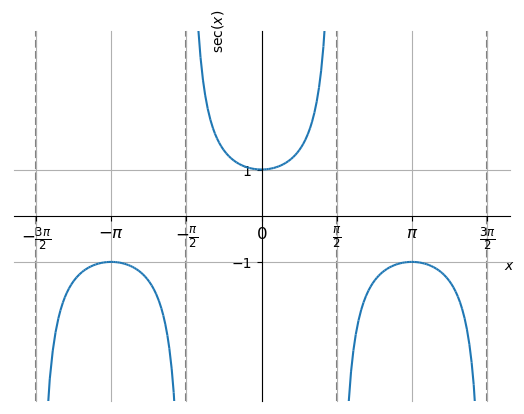
\includegraphics[width=0.5\textwidth]{./cap_funcao/dados/fig_co_sec_graficos/fig_sec_grafico}~
  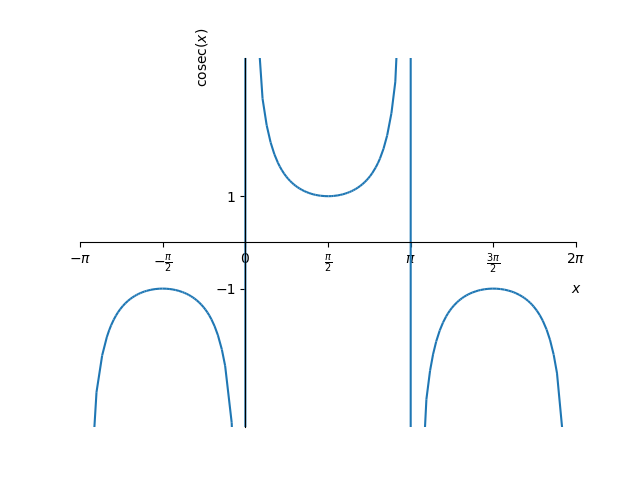
\includegraphics[width=0.5\textwidth]{./cap_funcao/dados/fig_co_sec_graficos/fig_cosec_grafico}
  \caption{Esboços dos gráficos das funções tangente (esquerda) e cotangente(direita).}
  \label{fig:co_sec_graficos}
\end{figure}

\subsection{Identidades trigonométricas}

Aqui, vamos apresentar algumas identidades trigonométricas que serão utilizadas ao longo do curso de cálculo. Comecemos pela identidade fundamental
\begin{equation}
  \sen^2 x + \cos^2 x = 1.
\end{equation}
Desta decorrem as identidades
\begin{align}
  &\tg^2(x) + 1 = \sec^2 x,\\
  &1 + \cotg^2(x) = \cosec^2(x).
\end{align}

Das seguintes fórmulas para adição/subtração de ângulos
\begin{align}
  &\cos(x\pm y) = \cos(x)\cos(y) \mp \sen(x)\sen(y),\\
  &\sen(x\pm y) = \sen(x)cos(y) \pm \cos(x)\sen(y),
\end{align}
seguem as fórmulas para ângulo duplo
\begin{align}
  &\cos(2x) = \cos^2x - \sen^2x,\\
  &\sen(2x) = 2\sen x\cos x.
\end{align}

Também, temos as fórmulas para o ângulo metade
\begin{align}
  &\cos^2 x = \frac{1 + \cos 2x}{2},\\
  &\sen^2 x = \frac{1 - \cos 2x}{2}.\label{eq:id_trig_cos_x2}
\end{align}

\subsection*{Exercícios}

\emconstrucao

\section{Operações com funções}\label{cap_funcao_sec_opfun}

\subsection{Somas, diferenças, produtos e quocientes}

Sejam dadas as funções $f$ e $g$ com domínio em comum $D$. Então, definimos as funções
\begin{itemize}
\item $(f\pm g)(x) := f(x) \pm g(x)$ para todo $x\in D$;
\item $(fg)(x) := f(x)g(x)$ para todo $x\in D$;
\item $\displaystyle \left(\frac{f}{g}\right)(x) := \frac{f(x)}{g(x)}$ para todo $x\in D$ tal que $g(x)\neq 0$.
\end{itemize}

\begin{ex}
  Sejam $f(x)=x^2$ e $g(x)=x$. Temos:
  \begin{itemize}
  \item $(f+g)(x) = x^2 + x$ e está definida em toda parte.
  \item $(g-f)(x) = x - x^2$ e está definida em toda parte.
  \item $(fg)(x) = x^3$ e está definida em toda parte.
  \item $\left(\frac{f}{g}\right)(x) = \frac{x^2}{x}$ e tem domínio $(-\infty, \infty)\setminus \{0\}$\footnote{Observemos que não podemos simplificar o $x$, pois a função $y=x$ é diferente da função $y=x^2/x$.}.
  \end{itemize}
\end{ex}

\subsection{Funções compostas}

Sejam dadas as funções $f$ e $g$. Definimos a {\bf função composta}\index{função!composta} de $f$ com $g$ por
\begin{equation}
  (f\circ g)(x) := f(g(x)).
\end{equation}
Seu domínio consiste dos valores de $x$ que pertençam ao domínio da $g$ e tal que $g(x)$ pertença ao domínio da $f$.

\begin{ex}
  Sejam $f(x) = x^2$ e $g(x) = x+1$. A função composta $(f\circ g)(x) = f(g(x)) = f(x+1) = (x+1)^2$.
\end{ex}

\subsection{Translações, contrações, dilatações e reflexões de gráficos}

Algumas operações com funções produzem resultados bastante característico no gráfico de funções. Com isso, podemos usar estas operações para construir gráficos de funções mais complicadas a partir de funções básicas.

\subsection{Translações}

Dada uma função $f$ e uma constante $k\neq 0$, temos que a o gráfico de $y = f(x) + k$ é uma translação vertical do gráfico de $f$. Se $k>0$, observamos uma translação vertical para cima. Se $k<0$, observamos uma translação vertical para baixo.

Translações horizontais de gráficos podem ser produzidas pela soma de uma constante não nula ao argumento da função. Mais precisamente, dada uma função $f$ e uma constante $k\neq 0$, temos que o gráfico de $y=f(x+k)$ é uma translação horizontal do gráfico de $f$ em $k$ unidades. Se $k>0$, observamos uma translação horizontal para a esquerda. Se $k<0$, observamos uma translação horizontal para a direita.

\subsection{Dilatações e contrações}

Sejam dados uma função $f$ e uma constante $\alpha$. Então, o gráfico de:
\begin{itemize}
\item $y = \alpha f(x)$ é uma dilatação vertical do gráfico de $f$, quando $\alpha > 1$;
\item $y = \alpha f(x)$ é uma contração vertical do gráfico de $f$, quando $0<\alpha < 1$;
\item $y = f(\alpha x)$ é uma contração horizontal do gráfico de $f$, quando $\alpha > 1$;
\item $y = f(\alpha x)$ é uma dilatação horizontal do gráfico de $f$, quando $\alpha < 1$.
\end{itemize}

\subsection{Reflexões}

Seja dada uma função $f$. O gráfico da função $y = -f(x)$ é uma reflexão em torno do eixo $x$ do gráfico da função $f$. Já, o gráfico da função $y = f(-x)$ é uma reflexão em torno do eixo $y$ do gráfico da função $f$.

\subsection*{Exercícios}

\emconstrucao

\section{Propriedades de funções}\label{cap_funcao_sec_prop}

\subsection{Funções crescentes ou decrescentes}

Uma da função $f$ é dita crescente quando $f(x_1)<f(x_2)$ para todos $x_1<x_2$ no seu domínio. É dita não decrescente quando $f(x_1)\leq f(x_2)$ para todos os $x_1<x_2$ no seu domínio. Analogamente, é dita decrescente quando $f(x_1)>f(x_2)$ para todos $x_1<x_2$. E, por fim, é dita não crescente quando $f(x_1)\geq f(x_2)$ para todos $x_1<x_2$, sempre no seu domínio.

\begin{ex}
  Vejamos os seguintes casos:
  \begin{itemize}
  \item A {\bf função identidade}\index{função!identidade} $f(x)=x$ é crescente.
  \item A função exponencial $f(x)=e^{-x}$ é decrescente.
  \item A seguinte função definida por partes
    \begin{equation}
      f(x) = \left\{
        \begin{array}{ll}
          x+1 &,x\leq 0,\\
          2 &,0<x\leq 1,\\
          (x-1)^2+2 &, x>1
        \end{array}
\right.
\end{equation}
é não decrescente.
  \end{itemize}
\end{ex}

\subsection{Funções pares ou ímpares}

Uma dada {\bf função} $f$ é dita {\bf par}\index{função!par} quando $f(x)=f(-x)$ para todo $x$ no seu domínio. Ainda, é dita {\bf ímpar}\index{função!ímpar} quando $f(x)=-f(-x)$ para todo $x$ no seu domínio.

\begin{ex}
  Vejamos os seguintes casos:
  \begin{itemize}
  \item $f(x) = x^2$ é uma função par.
  \item $f(x) = x^3$ é uma função par.
  \item $f(x) = \sen x$ é uma função ímpar.
  \item $f(x) = \cos x$ é uma função par.
  \item $f(x) = x+1$ não é par nem ímpar.
  \end{itemize}
\end{ex}

\subsection{Funções injetoras}

Uma dada {\bf função} $f$ é dita {\bf injetora} quando $f(x_1)\neq f(x_2)$ para todos $x_1\neq x_2$ no seu domínio.

\begin{ex}
  Vejamos os seguintes casos:
  \begin{itemize}
  \item $f(x) = x^2$ não é uma função injetora.
  \item $f(x) = x^3$ é uma função injetora.
  \item $f(x) = e^x$ é uma função injetora.
  \end{itemize}
\end{ex}

Função injetoras são funções invertíveis. Mais precisamente, dada uma função injetora $y = f(x)$, existe uma única função $g$ tal que
\begin{equation}
  g(f(x)) = x,
\end{equation}
para todo $x$ no domínio da $f$. Tal função $g$ é chamada de {\bf função inversa}\index{função!inversa} de $f$ é comumente denotada por $f^{-1}$.\footnote{Observe que, em geral, $f^{-1} \neq \frac{1}{f}$.}

\begin{ex}
  Vamos calcular a função a função inversa de $f(x) = x^3 + 1$. Para tando, escrevemos
  \begin{equation}
    y = x^3 + 1.
  \end{equation}
  Então, isolando $x$, temos
  \begin{equation}
    x = \sqrt[3]{y - 1}.
  \end{equation}
  Desta forma, concluímos que $f^{-1}(x) = \sqrt[3]{x-1}$. Verifique que $f^{-1}(f(x)) = x$ para todo $x$ no domínio de $f$!
\end{ex}

\begin{obs}
 Os gráficos de uma dada função injetora $f$ e de sua inversa $f^{-1}$ são simétricos em relação a {\bf reta identidade}\index{reta!identidade} $y=x$.
\end{obs}

\subsection*{Exercícios}

\emconstrucao

\section{Funções exponenciais}\label{cap_funcao_sec_funexp}

Uma {\bf função exponencial}\index{função!exponencial} tem a forma
\begin{equation}
  f(x) = a^x,
\end{equation}
onde $a\neq 1$ é uma constante positiva e é chamada de {\bf base}\index{base} da função exponencial.

Funções exponenciais estão definidas em toda parte e têm imagem $(0, \infty)$. O gráfico de uma função exponencial sempre contém os pontos $(-1,1/a)$, $(0,1)$ e $(1,a)$. Veja a Figura \ref{fig:exponencial_graficos}.

\begin{figure}[H]
  \centering
  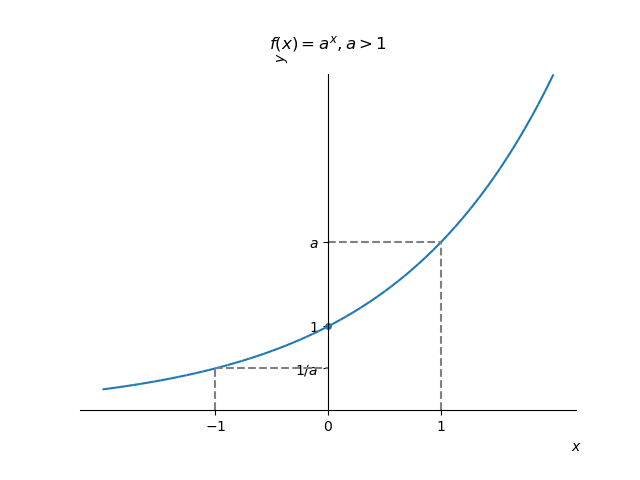
\includegraphics[width=0.5\textwidth]{./cap_funcao/dados/fig_exponencial_graficos/fig_exponencial_2}~
  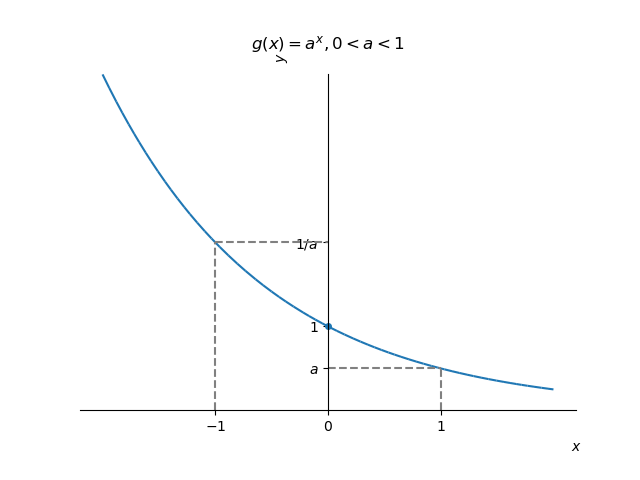
\includegraphics[width=0.5\textwidth]{./cap_funcao/dados/fig_exponencial_graficos/fig_exponencial_12}
  \caption{Esboços dos gráficos de funções exponenciais: (esquerda) $f(x) = a^x$, $a>1$; (direita) $g(x) = a^x$, $0<a<1$.}
  \label{fig:exponencial_graficos}
\end{figure}

\begin{obs}
  Quando a base é o número de Euler $e \approx 2,718281828459045$, chamamos $f(x) = e^x$ de função exponencial natural.

  \ifispython
  No \href{https://www.sympy.org}{SymPy}, o número de Euler é obtido com a constante \verb+E+:
\begin{verbatim}
>>> float(E)
2.718281828459045
\end{verbatim}
  \fi
\end{obs}

\subsection*{Exercícios}

\emconstrucao

\section{Funções logarítmicas}\label{cap_funcao_sec_funlog}

A {\bf função logarítmica}\index{função!logarítmica} $y = \log_a x$, $a>0$ e $a\neq 1$, é a função inversa da função exponencial $y = a^x$. Veja a Figura \ref{fig:log_graficos}. O domínio da função logarítmica é $(0,\infty)$ e a imagem $(-\infty, \infty)$.

\begin{figure}[H]
  \centering
  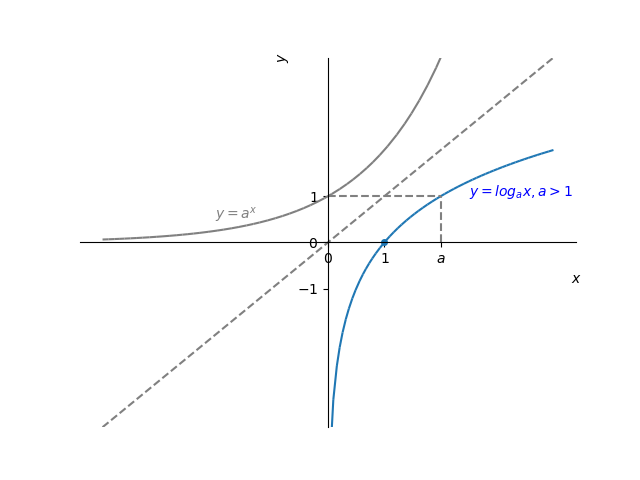
\includegraphics[width=0.5\textwidth]{./cap_funcao/dados/fig_log_graficos/fig_log_2}~
  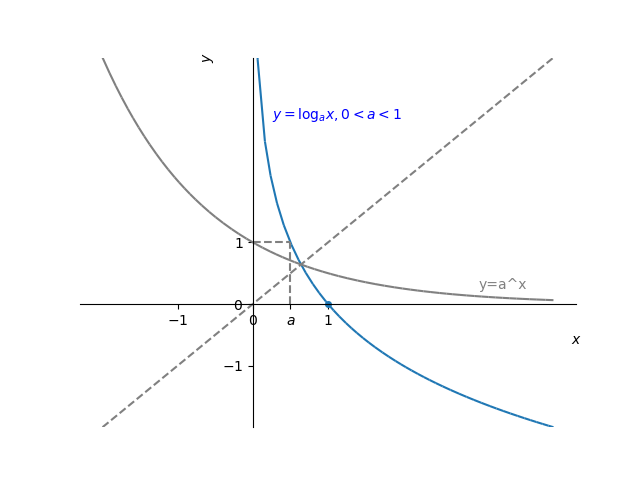
\includegraphics[width=0.5\textwidth]{./cap_funcao/dados/fig_log_graficos/fig_log_12}
  \caption{Esboços dos gráficos de funções logarítmicas: (esquerda) $y = \log_a x$, $a>1$; (direita) $y = \log_a x$, $0<a<1$.}
  \label{fig:log_graficos}
\end{figure}

\begin{obs}
  Quando a base é o número de Euler $e \approx 2,718281828459045$, chamamos $y = \log_e x$ de função exponencial natural e denotamo-la por $y = \ln x$.

  \ifispython
  No \href{https://www.sympy.org}{SymPy}, podemos computar $\log_a x$ com a função \verb+log(x,a)+. O $\ln x$ é computado com $\verb+log(x)+$.
  \fi
\end{obs}

\begin{obs}
  Vejamos algumas propriedades dos logaritmos:
  \begin{itemize}
  \item $\log_a x = y \Leftrightarrow a^y = x$;
  \item $\log_a 1 = 0$;
  \item $\log_a a = 1$;
  \item $\log_a a^x = x$;
  \item $a^{\log_a^x} = x$;
  \item $\log_a xy = \log_a x + \log_a y$;
  \item $\log_a \frac{x}{y} = \log_a x - \log_a y$;
  \item $\log_a x^r = r\cdot\log_a x$.
  \end{itemize}
\end{obs}

\subsection*{Exercícios}

\emconstrucao